\documentclass{article}%
\usepackage[a4paper, total={6in, 8in}]{geometry}

\usepackage{hyperref}
\usepackage[fleqn]{amsmath}
\usepackage{xcolor}
\usepackage{mathtools, nccmath}
\usepackage{algorithm}
\usepackage[noend]{algpseudocode}
\usepackage{graphicx}
\usepackage{listings}
\lstset{basicstyle=\ttfamily,
  showstringspaces=false,
  commentstyle=\color{red},
  keywordstyle=\color{blue}
}
\graphicspath{ {./images/}  }


\title{Parallelized Incompressible Navier-Stokes Equations Solvers in a Modern C++ Framework}
\date{July 22, 2019}
\author{Christoph Neuhauser\\ Computer Science, Technical University of Munich 
\and Stefan Haas\\ Computer Science, Technical University of Munich
\and Kwok Ping Ng\\ Data Engineering and Analytics, Technical University of Munich}
\begin{document}
\maketitle

\section{Introduction}

After studying the incompressible Navier-Stokes equations in 2D in the practical course, our goal was to implement the incompressible Navier-Stokes equations in 3D as our group project. To replace the C framework from the practical course, a modern C++ framework was created. Our first step was to rewrite the momentum, continuity and energy equations. In 3D, it is necessary to add a third velocity component, called W. More information on the equations in 3D can be found in \cite{griebel}.

Another goal was to elaborate how the CFD solver could be parallelized in a very efficient way. For this, we chose to compare a solver written in C++ with OpenMP (short: cpp solver), a solver using MPI for distributed-memory parallelism, a solver using CUDA on NVIDIA GPUs and a solver using OpenCL, which can be run on NVIDIA GPUs, Intel iGPUs and AMD GPUs. In the following section, we will describe the code and how to use it, as well as compare these solvers regarding their best performance results, their scalability and their parallel efficiency.

Finally, we simulated multiple scenarios like Rayleigh-Benard convection, and multiple real-world scenarios like the air flow around Mt. Fuji in Japan or the German mountain Zugspitze

\section{Code description}
\subsection{Code framwork}
The C++ Code is structured as follows. In the source directory in the file main.cpp, the main function is defined where the core of the program resides, which is basically of the same structures as the 2D CFD code. Furthermore, there also is the Defines.hpp file, which defines the floating-point precision (float or double) as well as some define statements for the mapping 3D indices in the staggered grid to 1D array indices. We couldn't use multi-dimensional arrays directly, as they aren't supported by CUDA and OpenCL.

Then there is the IO folder which contains everthing that has to do with input and output functionality, among others the VTK writer as well as the NetCDF writer and some classes to read and process different input formats for the geometry.

The folder ParticleTracer contains classes for tracing the characteristic lines of the flow. However, in the end we didn't use them for our simulation, as we decided to directly use ParaView for tracing the particles and omitted the idea for time reasons to use a program Christoph created for visualizing large line sets created by our application.

The most important part of the program is the CdfSolver folder, where all solvers as well as the solver interface is located. The interface defines the following methods:\pagebreak

\begin{lstlisting}[language=C++,frame=single]
void initialize(
    const std::string &scenarioName,
    LinearSystemSolverType linearSystemSolverType,
    bool shallWriteOutput, Real Re, Real Pr, Real omg, Real eps,
    int itermax, Real alpha, Real beta, Real dt, Real tau,
    Real GX, Real GY, Real GZ, bool useTemperature, Real T_h, Real T_c,
    int imax, int jmax, int kmax, Real dx, Real dy, Real dz,
    Real *U, Real *V, Real *W, Real *P, Real *T, uint32_t *Flag)
\end{lstlisting}
which copies the passed initial values of U, V, W, P, T and Flag to the internal representation of the solver.

\begin{lstlisting}[language=C++,frame=single]
void setBoundaryValues()
\end{lstlisting}
which sets the boundary condition values of U, V, W and T using the Flag array.

\begin{lstlisting}[language=C++,frame=single]
void setBoundaryValuesScenarioSpecific()
\end{lstlisting}
which sets special boundary conditions (typically something like inflow) specific to the different scenarios.

\begin{lstlisting}[language=C++,frame=single]
Real calculateDt()
\end{lstlisting}
which calculates the smallest possible (plus some safety margin) time step for the simulation at the current state.

\begin{lstlisting}[language=C++,frame=single]
void calculateTemperature()
\end{lstlisting}
which updates the temperature values (using an intermediate copy of the temperature from the last iteration).

\begin{lstlisting}[language=C++,frame=single]
void calculateFgh()
\end{lstlisting}
which computes the values in the helper arrays F, G and H necessary to compute the right-hand side of the Pressure.

\begin{lstlisting}[language=C++,frame=single]
void calculateRs()
\end{lstlisting}
which computes the right-hand side of the Pressure Poisson Equation (PPE).

\begin{lstlisting}[language=C++,frame=single]
void executeSorSolver()
\end{lstlisting}
which executes the SOR solver (successive over-relaxation) for solving the Pressure Poisson Equation (PPE).

\begin{lstlisting}[language=C++,frame=single]
void calculateUvw()
\end{lstlisting}
which updates the values in the arrays U, V and W.

\begin{lstlisting}[language=C++,frame=single]
void getDataForOutput(Real *U, Real *V, Real *W, Real *P, Real *T)
\end{lstlisting}
which copies the values of the internal representations of U, V, W, P and T to the specified arrays. This is necessary when outputting the simulation results at certain time intervals. This function abstracts the process of either copying the values of the internal representation in VRAM on GPUs when using CUDA or OpenCL to the main memory or copying the values of the internal representation of the MPI and OpenMP solvers in main memory to the representation in the main function also in main memory.

The CfdSolver directory also features classes to work with the flag array as well as to initialize the arrays for the different variables.

Finally, as sub-folders of the CfdSolver folder, there are the different folders which contain the individual solvers. Each solver has the same basic structure even though some have additional files and classes for different functions. Each solver has a file to manage the boundary values, the actual CfdSolver class, which mostly initializes variables and calls the function or kernels of the other files, the SOR solver file, where the SOR, Jacobi and/or the Gauss-Seidel solver are defined and finally the UVW file, which calculates everything what has to do with u, v and w, the temperature, or the timestep.

\subsection{Building the code}
The program is compiled with cmake. In order to build it, some packages have to installed (see the README file for more information on how to install them on Ubuntu) and the following commands have to be issued within the repository directory:
\begin{lstlisting}[language=bash,frame=single]
mkdir build
cd build
cmake ..
make
\end{lstlisting}

In order to use the different solvers, some arguments have to be given to cmake.
\begin{itemize}
\item For MPI support: cmake .. -DUSE\_MPI=ON
\item For CUDA support: cmake .. -DUSE\_CUDA=ON
\item For OpenCL support: cmake .. -DUSE\_OPENCL=ON
\end{itemize}
These arguments can also be used together for the program to support multiple solvers at once.

\subsection{Running the program}
When executing the program, multiple arguments can be passed on the command line. These arguments are shown in the following list as well as their respective valid values.
\begin{itemize}
\item scenario:
	\begin{itemize}
	\item driven\_cavity
	\item flow\_over\_step
	\item natural\_convection
	\item rayleigh\_benard\_convection\_8-2-1
	\item rayleigh\_benard\_convection\_8-2-2
	\item rayleigh\_benard\_convection\_8-2-4
	\item rayleigh\_benard\_convection\_2d
	\item single\_tower
	\item fuji\_san
	\item zugspitze
	\end{itemize}
\item solver:
	\begin{itemize}
	\item cpp
	\item mpi
	\item cuda
	\item opencl
	\end{itemize}
\item outputformat:
	\begin{itemize}
	\item netcdf
	\item vtk (= vtk-binary)
	\item vtk-binary
	\item vtk-ascii
	\end{itemize}
\item output:
	\begin{itemize}
	\item true
	\item false (whether to write an output file)
	\end{itemize}
\item linsolver:
	\begin{itemize}
	\item jacobi
	\item sor
	\item gauss-seidel
	\end{itemize}
\item tracestreamlines:
	\begin{itemize}
	\item false
	\item true
	\end{itemize}
\item tracestreaklines:
	\begin{itemize}
	\item false
	\item true
	\end{itemize}
\item tracepathlines:
	\begin{itemize}
	\item false
	\item true
	\end{itemize}
\item numparticles:
	\begin{itemize}
	\item any positive integer number
	\end{itemize}
\item numproc
	\begin{itemize}
	\item Must be used with the MPI solver. Specifys the number of processes in x, y and z direction and must match the total number of MPI processes.
	\item possible values: positive integer positive integer positive integer
	\item example: --numproc = 2 2 2
	\end{itemize}
\item blocksize
	\begin{itemize}
	\item Can be used with the CUDA or the OpenCL solver. Specifys the block size in x, y and z direction.
	\item possible values: positive integer positive integer positive integer
	\item example: --blocksize = 4 4 4
	\end{itemize}
\item platformid
	\begin{itemize}
	\item Can be used with the OpenCL solver. Specifys the ID of the OpenCL platform to use. If the ID is not specified, it is set to zero. Which platform corresponds to which ID can be found outwith the command line tool 'clinfo'.
	\item possible values: integer
	\end{itemize}
\end{itemize}

\noindent The standard values for the arguments are:
\begin{itemize}
\item scenario: driven\_cavity
\item solver: cpp
\item outputformat: vtk
\item outputformat: true
\item linsolver: jacobi
\item tracestreamlines: false
\item tracestreaklines: false
\item tracepathlines: false
\item numparticles: 1000
\item blocksize: 8 8 4
\item platformid: 0
\end{itemize}

Here are some examples on how the code can be run:
\begin{lstlisting}[language=bash, frame=single]
./cfd3d --scenario driven_cavity --solver cpp
mpirun -np 8 ./cfd3d --solver mpi --numproc 2 2 2
./cfd3d --scenario driven_cavity --solver cuda
\end{lstlisting}





\section{3D Incompressible Navier-Stokes equation}
The flow of non-stationary incompressible viscous fluid is described by the three dimensional Navier-Stokes equations. The quantities are computed as u, v, w and F, G, H as x, y, z directions.

\subsection{3D Momentum equations}
\begin{equation}
\frac{\partial u}{\partial t} + \frac{\partial p}{\partial x} = 
\frac{1}{Re} \left( \frac{\partial^2 u}{\partial x^2} + \frac{\partial^2 u}{\partial y^2} + \frac{\partial^2 u}{\partial z^2} \right) - 
\frac{\partial(u^2)}{\partial x} -\frac{\partial (uv)}{\partial y} - 
\frac{\partial (uw)}{\partial z} +
g_x 
\end{equation}

\begin{equation}
\frac{\partial v}{\partial t} + \frac{\partial p}{\partial y} = 
\frac{1}{Re} \left( \frac{\partial^2 v}{\partial x^2} + \frac{\partial^2 v}{\partial y^2} + \frac{\partial^2 v}{\partial z^2} \right) - 
\frac{\partial(uv)}{\partial x} -\frac{\partial (v^2)}{\partial y} - 
\frac{\partial (vw)}{\partial z} +
g_y
\end{equation}

\begin{equation}
\frac{\partial w}{\partial t} + \frac{\partial p}{\partial z} = 
\frac{1}{Re} \left( \frac{\partial^2 w}{\partial x^2} + \frac{\partial^2 w}{\partial y^2} + \frac{\partial^2 w}{\partial z^2} \right) - 
\frac{\partial(uw)}{\partial x} -\frac{\partial (vw)}{\partial y} - 
\frac{\partial (w^2)}{\partial z} +
g_z
\end{equation}

\subsection{3D Continuity equation}
\begin{equation}
\frac{\partial u}{\partial x} + \frac{\partial v}{\partial y} + \frac{\partial w}{\partial z} = 0
\end{equation}

\subsection{Force F and velocity u calculation in x direction}
The velocity w was added to the calculations from the 2D case and then, the discretization for the derivatives of u, v and w have to be derived with respect to directions x, y and z, respectively. Below, the computation of F and u is exemplified. The computation of G, H and v, w is analogous. \\
\\
F:
\begin{equation}
\begin{split}
F_{i,j,k} =
u_{i,j,k} & + \delta t \Bigl(
\frac{1}{Re} \left( \left[\frac{\partial^2 u}{\partial x^2}\right]_{i,j,k} + \left[\frac{\partial^2 u}{\partial y^2}\right]_{i,j,k} + \left[\frac{\partial^2 u}{\partial z^2}\right]_{i,j,k} \right) - 
\left[\frac{\partial(u^2)}{\partial x}\right]_{i,j,k} -\left[\frac{\partial (uv)}{\partial y}\right]_{i,j,k} - 
\left[\frac{\partial (uw)}{\partial z}\right]_{i,j,k}\\
& + {g_x} - \frac{\beta}{2} \left( T^{(n+1)}_{i,j,k} + T^{(n+1)}_{i+1,j,k} \right) g_x \Bigr)\\
& i = 1,\ldots,imax-1; \quad j = 1,\ldots,jmax; \quad k = 1,\ldots,kmax
\end{split}
\end{equation}
u:\\
\begin{equation}
\begin{split}
u^{(n+1)}_{i,j,k} = & F^{(n)}_{i,j,k} - \frac{\delta t}{\delta x}\left(p^{(n+1)}_{i+1,j,k} - p^{(n+1)}_{i,j,k}\right)\\
& i = 1,\ldots,imax-1; \quad j = 1,\ldots,jmax; \quad k = 1,\ldots,kmax
\end{split}
\end{equation}

\subsection{Discretization for F}
The derivatives of the 3 directions are discretized as follows using the midpoint rules and the donor cells scheme (again, exemplified only for u).\\
\begin{equation}
\left[\frac{\partial^2 u}{\partial x^2}\right]_{i,j,k} =
\frac{u_{i+1,j,k} - 2u_{i,j,k} + u_{i-1,j,k}}{(\delta x)^2}
\end{equation}

\begin{equation}
\left[\frac{\partial^2 u}{\partial y^2}\right]_{i,j,k} =
\frac{u_{i,j+1,k} - 2u_{i,j,k} + u_{i,j-1,k}}{(\delta y)^2}
\end{equation}

\begin{equation}
\left[\frac{\partial^2 u}{\partial z^2}\right]_{i,j,k} =
\frac{u_{i,j,k+1} - 2u_{i,j,k} + u_{i,j,k-1}}{(\delta z)^2}
\end{equation}

\begin{equation}
\begin{split}
\left[\frac{\partial(u^2)}{\partial x}\right]_{i,j,k} = &
\frac{1}{\delta x}
\left(
	\left(\frac{u_{i,j,k}+u_{i+1,j,k}}{2}\right)^2 -
	\left(\frac{u_{i-1,j,k}+u_{i,j,k}}{2}\right)^2
\right) + \\
& \frac{\gamma}{\delta x}
\left(
	\frac{|u_{i,j,k}+u_{i+1,j,k}|}{2} \frac{(u_{i,j,k}-u_{i+1,j,k})}{2} -
	\frac{|u_{i-1,j,k}+u_{i,j,k}|}{2} \frac{(u_{i-1,j,k}-u_{i,j,k})}{2}
\right)
\end{split}
\end{equation}

\begin{equation}
\begin{split}
\left[\frac{\partial(uv)}{\partial y}\right]_{i,j,k} = &
\frac{1}{\delta y}
\left(
	\frac{(v_{i,j,k}+v_{i+1,j,k})}{2} \frac{(u_{i,j,k}+u_{i,j+1,k})}{2} -
	\frac{(v_{i,j-1,k}+v_{i+1,j-1,k})}{2} \frac{(u_{i,j-1,k}+u_{i,j,k})}{2}
\right) + \\
& \frac{\gamma}{\delta y}
\left(
	\frac{|v_{i,j,k}+v_{i+1,j,k}|}{2} \frac{(u_{i,j,k}-u_{i,j+1,k})}{2} -
	\frac{|v_{i,j-1,k}+v_{i+1,j-1,k}|}{2} \frac{(u_{i,j-1,k}-u_{i,j,k})}{2}
\right)
\end{split}
\end{equation}

\begin{equation}
\begin{split}
\left[\frac{\partial(uw)}{\partial z}\right]_{i,j,k} = &
\frac{1}{\delta z}
\left(
	\frac{(w_{i,j,k}+w_{i+1,j,k})}{2} \frac{(u_{i,j,k}+u_{i,j,k+1})}{2} -
	\frac{(w_{i,j,k-1}+w_{i+1,j,k-1})}{2} \frac{(u_{i,j,k-1}+u_{i,j,k})}{2}
\right) + \\
& \frac{\gamma}{\delta z}
\left(
	\frac{|w_{i,j,k}+w_{i+1,j,k}|}{2} \frac{(u_{i,j,k}-u_{i,j,k+1})}{2} -
	\frac{|w_{i,j,k-1}+w_{i+1,j,k-1}|}{2} \frac{(u_{i,j,k-1}-u_{i,j,k})}{2}
\right)
\end{split}
\end{equation}
\subsection{Energy equation and Discretization}
The energy equation in 3D and its discretization are given as follows.\\
\\
Energy Equation:\\
\begin{equation}
T^{(n+1)}_{i,j,k} = T^{(n)}_{i,j,k} +  \delta t \left(
\frac{1}{Re} \frac{1}{Pr} \left( \left[\frac{\partial^2 T}{\partial x^2}\right]_{i,j,k} + \left[\frac{\partial^2 T}{\partial y^2}\right]_{i,j,k} + \left[\frac{\partial^2 T}{\partial z^2}\right]_{i,j,k} \right) 
- 
\left[\frac{\partial(uT)}{\partial x}\right]_{i,j,k} -\left[\frac{\partial (vT)}{\partial y}\right]_{i,j,k} - 
\left[\frac{\partial (wT)}{\partial z}\right]_{i,j,k}
\right)
\end{equation}
Discretization:\\
\begin{equation}
\left[\frac{\partial^2 T}{\partial x^2}\right]_{i,j,k} =
\frac{T_{i+1,j,k} - 2T_{i,j,k} + T_{i-1,j,k}}{(\delta x)^2}
\end{equation}

\begin{equation}
\begin{split}
\left[\frac{\partial(uT)}{\partial x}\right]_{i,j,k} = &
\frac{1}{\delta x}
\left(
	u_{i,j,k} \frac{T_{i,j,k}+T_{i+1,j,k}}{2} -
	u_{i-1,j,k} \frac{T_{i-1,j,k}+T_{i,j,k}}{2}
\right) + \\
& \frac{\gamma}{\delta x}
\left(
	|u_{i,j,k}| \frac{T_{i,j,k}-T_{i+1,j,k}}{2} -
	|u_{i-1,j,k}| \frac{T_{i-1,j,k}-T_{i,j,k}}{2}
\right)
\end{split}
\end{equation}
\subsection{SOR Solver}
Pressure:\\
\begin{equation}
\begin{split}
p^{it+1}_{i,j,k} = & (1 - \omega) p^{it}_{i,j,k} + \frac{\omega}{2 (\frac{1}{(\delta x)^2} + \frac{1}{(\delta y)^2} + \frac{1}{(\delta z)^2})} \left( \frac{p^{it}_{i+1,j,k} + p^{it+1}_{i-1,j,k}}{(\delta x)^2} + \frac{p^{it}_{i,j+1,k} + p^{it+1}_{i,j-1,k}}{(\delta y)^2} + \frac{p^{it}_{i,j,k+1} + p^{it+1}_{i,j,k-1}}{(\delta z)^2} - rs_{i,j,k} \right)\\
& it = 1,\ldots,itmax; \quad i = 1,\ldots,imax; \quad j = 1,\ldots,jmax; \quad k = 1,\ldots,kmax
\end{split}
\end{equation}
Residual:\\
\begin{equation}
\begin{split}
res := & \left( \sum_{i=1}^{imax} \sum_{j=1}^{jmax} \sum_{k=1}^{kmax} \left( \frac{p_{i+1,j,k} - 2 p_{i,j,k} + p_{i-1,j,k}}{(\delta x)^2} + \frac{p_{i,j+1,k} - 2 p_{i,j,k} + p_{i,j-1,k}}{(\delta y)^2} + \frac{p_{i,j,k+1} - 2 p_{i,j,k} + p_{i,j,k-1}}{(\delta z)^2} \right. \right. \\
& \left. \left. - rs_{i,j,k} \right)^2 / (imax \cdot jmax \cdot kmax) \right)^{1/2}
\end{split}
\end{equation}
\section{Boundary Conditions}
\subsection{No Slip} 
When using no-slip conditions, zero velocities are imposed at the boundaries. In the staggered grid, it may be necessary to set the negaitve value at the boundary from within the domain, as averaging the values on both sides of the boundary would then give exactly zero. For example, in the left wall case we have: $u_{0,j,k}$ = 0 ,$v_{0,j,k}$ = -$v_{1,j,k}$, $w_{0,j,k}$ = -$w_{1,j,k}$.
\subsection{Free Slip} 
Free-slip means that the fluid can flow freely parallel to the boundarym but cannot have a perpendicular flow component at the boundary. In 3D cases, the fluid freely flows along two dimension, but cannot flow along the remaining direction. For example, the velocity at the left wall is imposed to be 0. Its boundary values are set to $u_{0,j,k}$ = 0, $v_{0,j,k}$ = $v_{1,j,k}$, and $w_{0,j,k}$ = $w_{1,j,k}$. For more details see figure~\ref{fig:boundaryConditions} below.

\begin{figure}[htb]
\centering
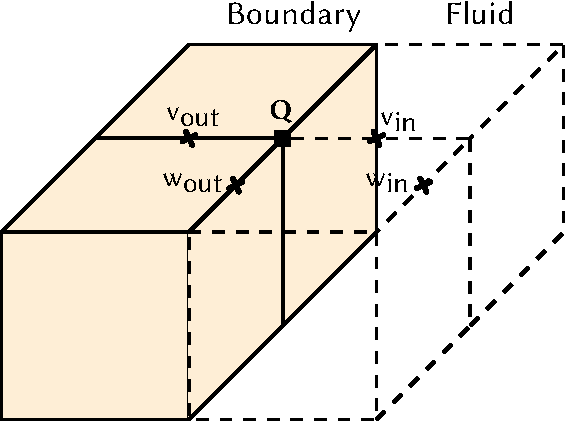
\includegraphics[width=0.4\linewidth]{images/BoundaryConditions.pdf}
\caption{Boundary conditions for an obstacle wall on the left.}
\label{fig:boundaryConditions}
\end{figure}

\subsection{Outflow}
For the outflow boundary condition, the normal velocity derivatives are set to 0 at the boundary. This means that the total velocity does not change in the direction normal to the boundary. The values of velocities at boundaries can be set equal to the neighbouring velocities inside the region. For example, in the left wall case we have: $u_{0,j,k}$ = $u_{1,j,k}$ ,$v_{0,j,k}$ = $v_{1,j,k}$, $w_{0,j,k}$ = $w_{1,j,k}$
\subsection{Boundary conditions for pressure and temperature}
The boundary conditions for the pressure are derived from the momentum equation and result in discrete Neumann conditions. The boundary conditions for the temperature, on the other hand, are derived from the energy equation and result in discrete Dirichlet boundary conditions for cold walls and hot walls, respectively. For example, in the left wall case we have: $P_{0,j,k}$ = $P_{1,j,k}$.  $T_{0,j,k}$ = $2*T_c/T_h$ – $T_{1,j,k}$.

\section{Performance}
\subsection{CUDA}
First of all, on consumer hardware, the CUDA solver and the OpenCL solver had considerable advantages over the CPU solvers. The results can be seen in figure~\ref{fig:platforms}, which where generated on a NVIDIA GeForce GTX 1070, a 6-core Intel Core i7-8700 and on a 28-core Intel Xeon E5-2697 from the Linux Cluster of the LRZ. Graphics cards offer a much higher number of cores available for applications to utilize compared to similar prized-processors. However, GPUs execute workloads in a SIMD-fashion in lockstep, which means that a thread warp (that usually consists of 32 or 64 individual threads) would need to go the same route in the code without any diverging branches to reach the maximum possible performance. Furthermore, another problem is that especially NVIDIA limits their double-precision performance on consumer-level graphics cards to create an additional sales rationale for their high-priced workstation cards.

In theory, according to \cite{cuda-guide}, the throughput of arithmetic double-precision floating point instructions on the GTX 1070 would be 1 : 32. However, the CUDA solver proved to be only approximately 48\text{\%} slower in our test case for double-precision floating point values compared to single-precision floating point values, which can be seen in figure~\ref{fig:platforms}. This can probably be attributed to the application being memory throughput limited for floating point operations rather than being limited by the throughput of arithmetic instructions.

On modern CPU architectures, the floating point units (FPUs) don’t offer separate modules for single-precision and double-precision instructions anymore. Thus, as expected, the CPU solvers were only approximately 2\text{\%} slower for double-precision floating-point numbers compared to single-precision floating-point numbers in our test case. The slight reduce in performance can probably also be attributed to the higher memory throughput caused by 64-bit wide double-precision floating-point numbers.

\subsection{MPI}
When comparing the scalability of the solvers, it is of course evident that the MPI solver offers the best scalability, as a memory-distributed program can be scaled to an arbitrary amount of cores. The weakness of the MPI solver comes into play when comparing it to a shared-memory implementation of the CFD solver on systems with a moderate number of cores. On our 6-core test system, the MPI solver was approximately 35\text{\%} slower than the OpenMP solver. Figure~\ref{fig:platforms} shows this difference. This is of course due to the communication overhead for the MPI solver. The advantage of MPI comes into play when utilizing multiple nodes of a cluster at once with distributed memory.
When using two nodes and 56 cores, the MPI solver (with a domain decomposition of 7x4x2) gave by far the best performance results of all CPU solvers, but the CUDA solver still was 85\text{\%} faster on the NVIDIA GeForce GTX 1070 even when comparing double-precision performance. There are probably two reasons for that. First of all, we used strong scaling with a fixed global problem size of 80x20x10 cells. It is of course comprehensible that the overhead for communication becomes really large for this high number of processes and a small local domain size. Secondly, the CUDA solver is able to very efficiently utilize the SIMD functionality of the GPU to provide a really large number of threads accessing very fast shared GDDR5 memory without almost any communication overhead.

\begin{figure}[htb]
\centering
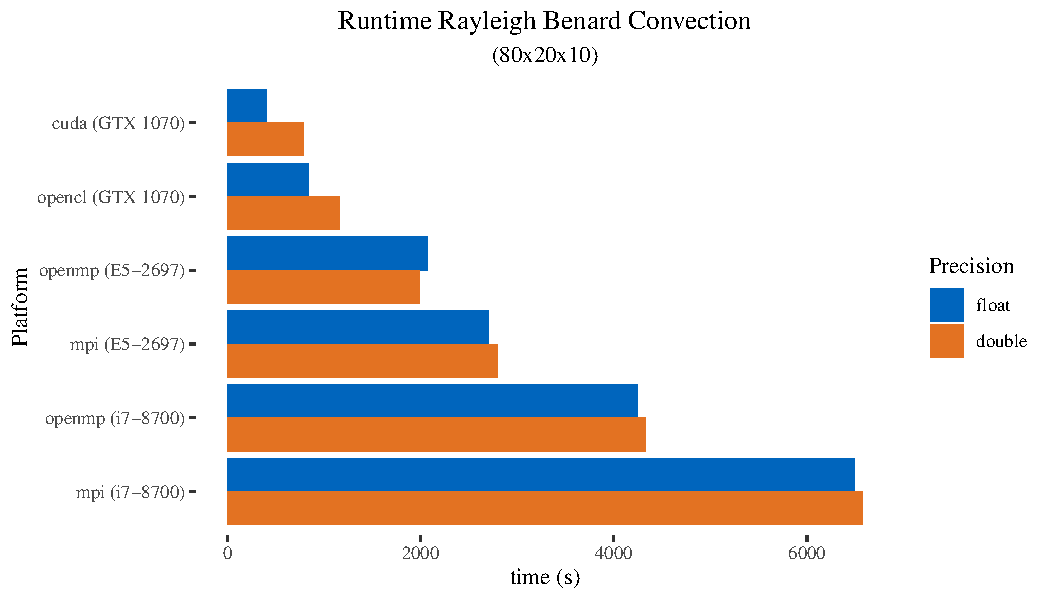
\includegraphics[width=1\linewidth]{../tests/graphs/runtime_rayleigh_benard_convection_8-2-1_platforms.pdf}
\caption{Performance results for different solvers. E2-2697: 28 cores, i7-8700: 6 cores. All results with Jacobi solver.}
\label{fig:platforms}
\end{figure}

\subsection{SOR and alternatives}
When parallelizing the CFD solver, it is also necessary to parallelize the solver used for the linear system of equations of the Pressure Poisson Equation (PPE).

For the parallel solvers, we decided to implement and compare a Jacobi, Gauss-Seidel (GS) and successive over-relaxation (SOR) solver. Each of the solvers has its own advantages and disadvantages.

Jacobi is the solver to converge slowest (measured by the number of iterations, not the runtime on multiple cores). However, its greatest advantage is that it can be easily parallelized, as it has no data dependencies within one iteration.

Gauss-Seidel converges in less iterations than Jacobi, but is harder to parallelize. The vanilla SOR algorithm without any adaptions generally cannot run in parallel. Thus, Gauss-Seidel only has an advantage over Jacobi when using a low number of cores. We tested the parallel SOR solver by Cunha and Hopkins \cite{parallel-sor}, but for sparse system matrices like in our case, the sequential update step in the end of the algorithm quickly becomes limiting for a high number of cores due to Amdahl’s law.

SOR is an algorithm based on Gauss-Seidel that couples the algorithm with an over-relaxation factor that can increase the convergence speed. In our program, we tested multiple values, and generally got the best results for an over-relaxation factor of 1.5. In our tests, which can be seen in figure~\ref{fig:solver}, Gauss-Seidel was faster than SOR, which is not what one might expect. However, when testing multiple over-relaxation factors, we noticed that the test scenario we chose (Rayleigh-Benard convection) needs a much lower over-relaxation factor than other scenarios. For an over-relaxation factor of 1.2, it performed slightly better than Gauss-Seidel. Again, SOR suffers from the same weakness as Gauss-Seidel that it can’t be parallelized easily. Thus, again, for a high number of cores, the Jacobi solver was able to beat the SOR solver.

Another method for solving a system of linear equations mentioned less often is the Jacobi over-relaxation (JOR), which transfers the principle of SOR to the Jacobi solver. However, for over-relaxation factors greater than 1, the solution would not converge. Thus, we rejected the JOR solver, as it can only increase convergence speed for a factor larger than 1. In the literature, we couldn’t find any other source having success with JOR coupled with a factor greater than 1.

Taking all factors mentioned above into account, we decided to select the Jacobi solver as the standard solver in our program, as it converges considerably faster in the same time compared to the SOR solver for a high number of cores. In figure~\ref{fig:solver} it can be seen that the difference between the solvers when using MPI is really small, since all solvers are parallelised (as the Gauss-Seidel scheme is replaced with a Jacobi scheme at the local domain boundaries of the processes for SOR and Gauss-Seidel). In the case of OpenMP, our tests show that our decision to use Jacobi was correct.

\begin{figure}[htb]
\centering
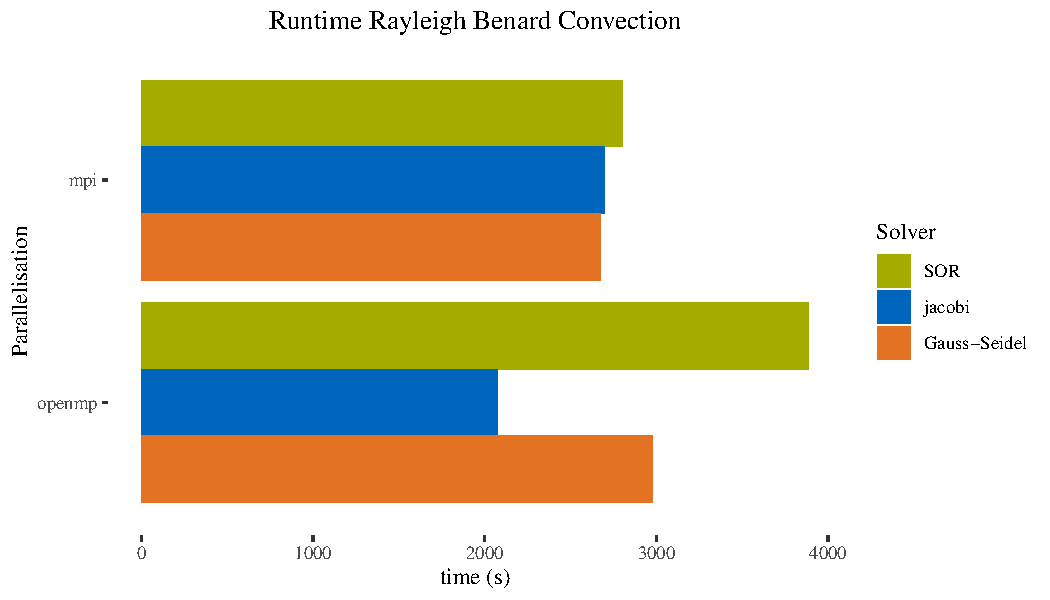
\includegraphics[width=1\linewidth]{../tests/graphs/runtime_rayleigh_benard_convection_8-2-1_solver.pdf}
\caption{All cases tested on a E2-2697 with 28 cores.}
\label{fig:solver}
\end{figure}


\subsection{Speedup}
After we chose the best solver, we tested the performance when using a different number of cores. These tests were run on the Linux Cluster of the LRZ, where we used one node with a Intel Xeon E5-2697 for the speedup tests with OpenMP and up to two nodes with the same processor for the speedup tests with MPI.

The results of the tests with OpenMP can be seen in figure~\ref{fig:speedup_openmp}. The speedup is exactly as we expected. At the beginning the performance scales very well while the speedup at the end degrades. At 28 cores the speedup is approximately 14.

To test the MPI implementation, we used one node for the first test. The reason we used 27 out of the 28 cores is that the domain could be split better with this amount of mpi processes, since the domain can be split in 3x3x3 parts, whereas with 28 processes it would be split into 7x2x2 part. We also tested both variants and the version with 27 processes was faster. With 27 cores the speedup is around ten, which is not as good as with OpenMP, but when using two nodes with 56 cores altogether, the performance scales almost linearly with an speedup of approximately 19, even though the domain is split in 7x4x2 parts, which is not optimal.


\begin{figure}[htbp]
\centering
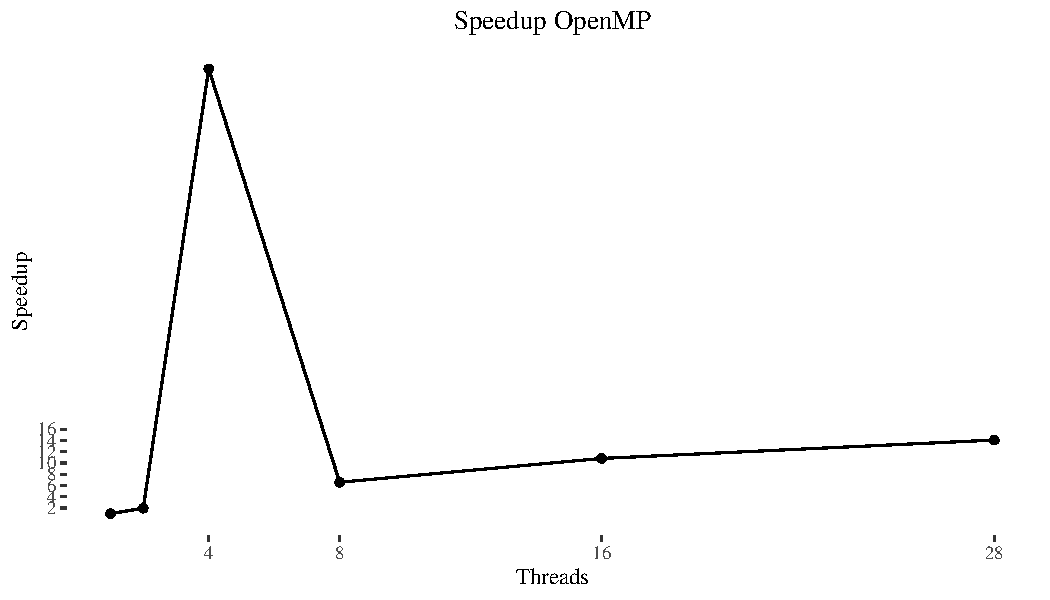
\includegraphics[width=1\linewidth]{../tests/graphs/speedup_OpenMP_double.pdf}
\caption{All cases tested on a E2-2697 with 28 cores.}
\label{fig:speedup_openmp}
\end{figure}

\begin{figure}[htbp]
\centering
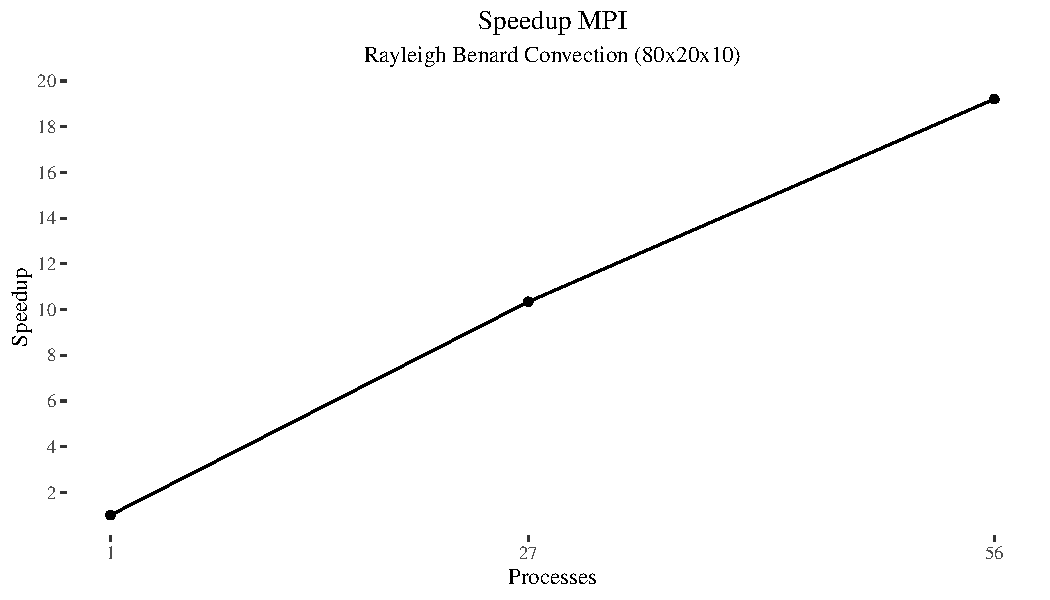
\includegraphics[width=1\linewidth]{../tests/graphs/speedup_MPI.pdf}
\caption{All cases tested on one or two nodes using a E2-2697 with 28 cores.}
\label{fig:speedup_MPI}
\end{figure}


\section{Arbitrary Geometries}
\subsection{u,v,w}

Unlike in the 2D cases, where it is necessary to set the arbitrary geometry boundary conditions for 8 directions (4 lines + 4 corners of a square), there are a total of 26 directions (12 edges, 8 corners and 6 faces of a cube) to be set. Setting the boundary values in 3D with the same method as utilized in worksheet 2 proved to be difficult.  Therefore, we designed a different approach to set the boundary conditions for arbitrary geometries.

We observed that we could set velocities lying right on the boundary to zero. Moreover, for the other values, the boundary value zero can be achieved by averaging the values on both sides of the boundary. This is an analogous case as when setting no-slip boundary condition on walls. We chose to set u, v and w separately. The direction flag is used to check if the velocity is lying on the wall. If it is, the velocity is set to zero. Then an indicator is inserted that this velocity may not be overwritten anymore. Otherwise, the velocity was set to equal the negative of the neighboring velocity. For example, below is pseudo code of the arbitrary geometry boundary conditions of u on the left wall.

\begin{algorithm}
\caption{Algorithm on the left boundary}\label{euclid}
\begin{algorithmic}
\For{over i,j,k}
	\State $a\gets 0$
	\State $b\gets 0$ 
	\If {Flag is not fluid}
    	\If {Left flag is obstacle}
    		\State $u_{i-1,j,k}\gets 0$
    		\State $a\gets 1$
    	\EndIf
    	\If {Up flag is obstacle}
    		\If {$a == 0$}
    			\State $u_{i-1,j,k}\gets -u_{i-1,j+1,k}$
    			\State $b\gets 1$
    		\EndIf	
    	\EndIf
    	\If {Down flag is obstacle}
    		\If {$a == 0$}
    			\State $u_{i-1,j,k}\gets -u_{i-1,j-1,k}$
    			\State $b\gets 1$
    		\EndIf	
    	\EndIf 
    	\If {Back flag is obstacle}
    		\If {$a == 0$ and $b==0$}
    			\State $u_{i-1,j,k}\gets -u_{i-1,j,k-1}$
    			\State $b\gets 1$
    		\EndIf	
    	\EndIf    	   	
    	\If {Front flag is obstacle}
    		\If {$a == 0$ and $b==0$}
    			\State $u_{i-1,j,k}\gets -u_{i-1,j,k+1}$
    			\State $b\gets 1$
    		\EndIf	
    	\EndIf       	
\EndIf
\EndFor
\end{algorithmic}
\end{algorithm}

\newpage

\subsection{Pressure and Temperature}
When setting the arbitrary geometry boundary conditions of pressure and temperature, the same methodology is used. As the pressure and temperature at the direction are the average of the values of the fluid neighbors involved, for example, \textit{B\_URF} (up, right and front)’s pressure is $P_{ijk} = (P_{i+1jk} + P_{ij+1k} + P_{ijk+1})/3$. So each flag of direction is checked separately and the values of the neighboring fluid cells are averaged.

\begin{algorithm}
\caption{Algorithm for pressure boundary conditions}\label{euclid}
\begin{algorithmic}
\For{over i,j,k}
	\State $numDirectFlag\gets 0$
	\State $P\_temp\gets 0$
	\If {Flag is not fluid}
    	\If {Left flag is obstacle}
    		\State $P\_temp += P_{i+1,j,k}$
    		\State $numDirectFlag++$
    	\EndIf
    \State{...}	    	
    \State $P_{i,j,k}= P\_temp / numDirectFlag$
\EndIf
\EndFor
\end{algorithmic}
\end{algorithm}



\begin{thebibliography}{999}
\bibitem{cuda-guide}
NVIDIA. 2019. CUDA C Programming Guide. \url{https://docs.nvidia.com/cuda/cuda-c-programming-guide/index.html#arithmetic-instructions} visited on 2019-07-18.
\bibitem{parallel-sor}
Rudnei Dias da Cunha, Tim Hopkins. 1991. Parallel Overrelaxation Algorithms for Systems of Linear Equations.
\bibitem{griebel}
M. Griebel, T. Dornseifer, and T. Neunhoeffer. SIAM, Philadelphia, 1998. Numerical Simulation in Fluid Dynamics, a Practical Introduction.
\end{thebibliography}

\end{document}